\documentclass[hidelinks,12pt,a4paper,openright,twoside]{book}
\usepackage[italian]{babel}
\usepackage[utf8]{inputenc}
\usepackage{fourier}

% Images
\usepackage{graphicx}
\usepackage{caption}
\usepackage{subcaption}
\usepackage{float}
\graphicspath{ {../Images} }

% Stop hyphenation
\usepackage[none]{hyphenat}

% Background page image.
\usepackage{eso-pic}
\usepackage[top=2cm, bottom=2cm, outer=0cm, inner=0cm]{geometry}

% To hide images
\usepackage[allfiguresdraft]{draftfigure}

% To color text parts
\usepackage{xcolor}

% License
\usepackage[
type={CC},
modifier={by-nc-sa},
version={4.0},
]{doclicense}

\begin{document}
	
	% Remove page number
	\pagestyle{empty}
	
	% Album Cover
	\begin{center}
		\vspace*{15mm}
		\fboxrule=4pt{
		\fbox{ %                  height                                width
			\begin{minipage}[l] [\dimexpr 0.150\textwidth \relax] [t] {\dimexpr .460\textwidth \relax}
				\vspace{5mm}
				\centering{\large \textbf{Album sulle opere del Museo Civico\\}}
				\bigskip
				Alice Balestieri \\
				Francesco Rombaldoni
			\end{minipage}
			}
		}
	\end{center}
	
	% Background image
	\AddToShipoutPictureBG*{\includegraphics[draft=false, width=\paperwidth,height=\paperheight]{example-image}}
	%\clearpage
	
	\newpage
	
		
			\begin{minipage}{\linewidth}
				\raggedright{
				\setdf{content={\textcolor{white}{1.}}}
				\hspace{15mm}\colorbox{black}{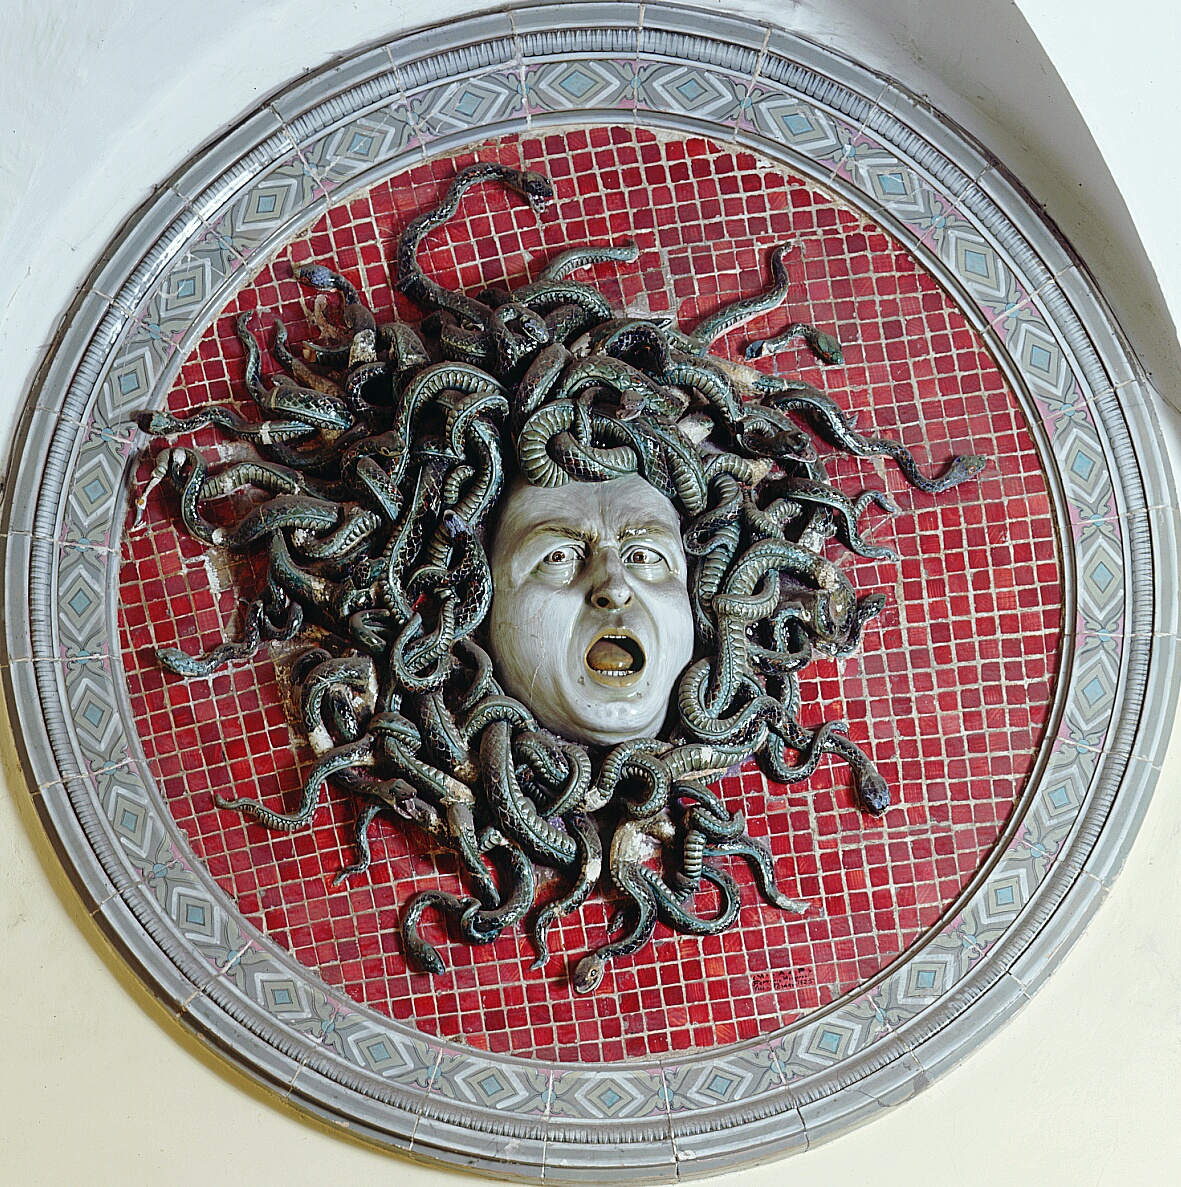
\includegraphics[]{Mengaroni_Ferruccio-Medusa.jpg}}
				\vspace{5mm}
				
				\begin{minipage}{0.4\linewidth}
					"La Medusa" accoglie i visitatori introducendoli alle sale espositive; si tratta dell'ultima opera di Ferruccio Mengaroni.\\
					L'imponente Medusa ritrae i lineamenti dell'artista pesarese: la leggenda narra che, per riprodurre il proprio volto, egli si fosse servito di uno specchio che poi si ruppe.
				\end{minipage}
			}
			\end{minipage}
		
	
\end{document}